\documentclass[tikz,border=10pt]{standalone}
\begin{document}
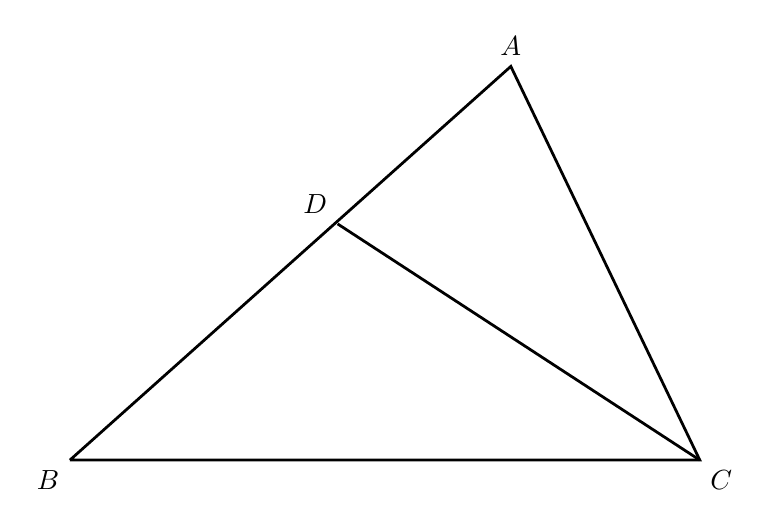
\begin{tikzpicture}[line width=1pt]

\coordinate (B) at (0,0);
\coordinate (C) at (8,0);
\coordinate (A) at (5.6,5.0);
\coordinate (D) at (3.4,3.0);

\draw (B) -- (A) -- (C) -- (B);
\draw (D) -- (C);

\node[below left] at (B) {$B$};
\node[below right] at (C) {$C$};
\node[above] at (A) {$A$};
\node[above left] at (D) {$D$};

\end{tikzpicture}
\end{document}
